% !TEX root = ../main.tex
\documentclass[../main.tex]{subfiles}
\begin{document}

\chapter{The dynamics of thermalisation in the Galerkin-truncated, three-dimensional Euler equation}
\label{trunc-euler}

% \begin{quote}
% \textit{C. Rajarshi$^{1}$, Mohammad Saif Khan$^{1}$, Prateek Anand$^{2}$, and Samriddhi Sankar Ray$^{1}$}\\[0.3em]
% \footnotesize
% $^{1}$International Centre for Theoretical Sciences, Tata Institute of Fundamental Research, Bangalore 560089, India\\
% $^{2}$Department of Mechanical Engineering, Indian Institute of Technology Bombay, Powai, Mumbai 400076, India
% \end{quote}

\begin{summary}
The {three-dimensional incompressible Euler equation}
when projected via a Galerkin-truncation on a finite-dimensional
subspace spanning wavenumbers $-{\bf K}_{\rm G} \le {\bf k} \le {\bf
K}_{\rm G}$, and hence retaining a finite number of modes $N_{\rm G}$,
lead to absolute equilibrium states. We review how this system
thermalises and its  connection to questions in turbulence. We also
discuss an emergent pseudo-dissipation range in the energy spectrum and
the time-scales associated with thermalisation.
\end{summary}

\section{Introduction}

Turbulent flows, with its tell-tale self-similar, intermittent, chaotic and
	multifractal signatures, are ubiquitous in the natural world~\cite{Frisch-Book}.
	%describe phenomena spanning from large scale winds, down to small scale dynamics of swimming bacteria \cite{Vallis06,mukherjee2023}}.
	For classical turbulence, such flows are solutions of the Navier-Stokes
	equation, with appropriate boundary conditions, forcing and small
	enough viscosities $\nu$, leading to driven-dissipative,
	non-equilibrium {statistically} stationary states which defy a Hamiltonian description.
	This lack of Hamiltonian description, among others, makes turbulence a particularly difficult problem, especially when viewed through
	the lens of statistical physics and field theory. However, for ideal,
	inviscid flows in the absence of forcing, would it be
	possible to uncover a Hamiltonian description~\cite{MorrisonRMP}?

The answer is delicate. Assuming incompressibility $\nabla\cdot\vec{u} = 0$ of
the  velocity field $\vec{u}$, and unit (constant) density, the Hamiltonian
\begin{equation}
\mathbb{H}[\vec{u}] = \frac{1}{2}\int |\vec{u}|^2 d{\bf x} \ ,
\end{equation}
leads to the three-dimensional (3D) Euler equation
through the Lie-Poisson bracket formalism where the pressure field $\mathcal{P}$ emerges as a Lagrange multiplier enforcing
the incompressibility constraint ~\cite{MorrisonRMP}.
In the rest of this paper, we will work in the space of periodic functions and {hence solutions --- numerical and theoretical --- of
the Euler equation will be considered on a 2$\pi$, triply-periodic cubic domain. This choice of the domain and boundary conditions,
together with incompressibility,
ensures that the invariants of the Euler equation --- namely, energy and helicity --- are conserved even in the truncated version
defined below.}

The Hamiltonian formulation runs into trouble when dealing with
\textit{weak} or dissipative solutions of the Euler equations:
\begin{equation}
\frac{\partial \vec{u}}{\partial t} + \vec{u}\cdot \nabla \vec{u} = -\nabla \mathcal{P} \ .
\label{thrm-eq:Euler}
\end{equation}
In particular, solutions with H\"older regularity {$h \le \nicefrac{1}{3}$} lead to non-conservation of
kinetic energy --- the problem of anomalous dissipation in turbulence~\cite{Eyink2024} --- and
hence the breakdown of a classical Hamiltonian structure.

Curiously, there is a form of the Euler equation which preserves its Hamiltonian structure~\cite{Lee1952} and conserves the kinetic energy. Let us chose a Galerkin wavevector ${\bf K}_{\rm G}$, such that the dynamics of the Euler
equation is restricted between wavevectors $-{\bf K}_{\rm G} \le {\bf k} \le {\bf K}_{\rm G}$ through
the self-adjoint, orthogonal, Hermitian Galerkin projector $\mathbb{P}_{{\bf K}_{\rm G}}$, defined as
{\begin{equation}
	{\bf u} \equiv \mathbb{P}_{{\bf K}_{\rm G}} \vec{u} = \sum_{{\bf k} = -{\bf K}_{\rm G}}^{{\bf k} = {\bf K}_{\rm G}} \hat{\vec{u}}_{\bf k} e^{i {\bf k}\cdot {\bf x}},
\label{thrm-eq:PG}
\end{equation}}
where $\hat{\vec{u}}_{\bf k}$ are the Fourier modes of the velocity field $\vec{u}({\bf x})$ obeying the untruncated Euler equation~\eqref{thrm-eq:Euler}, {and $i = \sqrt{-1}$}.
{The Galerkin truncation may in general be performed on different
finite-dimensional subsets of Fourier space. In this work we adopt the
standard sharp spherical truncation $|\mathbf{k}| \le K_{\rm G}$, which
preserves isotropy of the flow.}

In what follows, it will be useful to often work with the Fourier modes ${\bf \hat{u}_k}$ of the Galerkin-truncated velocity field $\bf u(x,t)$.
These obey, as easily derived from Eq.~\eqref{thrm-eq:Euler},
{\begin{equation}
	\frac{\partial {\bf \hat{u}_k}}{\partial t} + \sum_{\substack{{\bf p}+{\bf q}={\bf k}\\}}
	i  \left ({\bf k}\cdot{\bf \hat{u}_p}\right ){\bf \hat{u}_q}
	= -i {\bf k} {\hat{\mathcal{P}}}_{\bf k},
\label{thrm-eq:GTE_FS}
\end{equation}}
with $|{\bf p}|,|{\bf q}|,|{\bf k}|\le|{\bf K}_{\rm G}|$. This, then is the Fourier-space
representation~\cite{RayThermalReview2015} of the Galerkin-truncated, incompressible Euler equation
\begin{equation}
	\frac{\partial {\bf u}}{\partial t} + \mathbb{P}_{{\bf K}_{\rm G}}\left [{\bf u}\cdot \nabla {\bf u} + \nabla \mathcal{P} \right ] = 0,
\label{thrm-eq:GTE_RS}
\end{equation}
with initial conditions ${\bf u}_0 =  \mathbb{P}_{{\bf K}_{\rm G}}\vec{u}_0$.
For incompressible flows, these equations are augmented by the incompressibility constraint $\bf \nabla \cdot \bf u = 0$,  which is preserved by the Galerkin projector.

{The Galerkin-truncated velocity field ${\bf u}$ provides a natural way to define the
kinetic energy per unit mass $\mathbb{E} = \frac12\int |{\bf u}|^2 d{\bf x}/\int d{\bf x}$, helicity
$\mathcal{H} = \int {\bf u}\cdot(\boldsymbol{\nabla}\times{\bf u}) ~d{\bf x}$,
the isotropic energy spectrum $\mathbb{E}(k) = \sum_{k-1/2 < |\mathbf{k'}| \le k+1/2}
\frac{1}{2}|\hat {\bf u}_{\mathbf{k'}}|^2 $, and the kinetic energy flux  $\Pi(k) = \sum_{k' \ge k} T(k')$, where
the transfer term $T(k) = \partial_t \mathbb{E}(k)$, in a manner analogous
to what is done for the 3D Euler or indeed the Navier-Stokes equation.}

\section{Spectral signatures of thermalisation}
While a superficial comparison of the Galerkin-truncated equation with the
untruncated Euler equation may suggest that the two ought to be similar, it
turns out that the solutions $\vec{u}$ and ${\bf u}$ are markedly different.
While the Euler equation, given in Eq.~\eqref{thrm-eq:Euler}, is a partial
differential equation with an infinite number of modes, its Galerkin-truncated
version is finite-dimensional, with a fixed $N_{\rm G}$ number of modes{, and
thus a set of coupled ordinary differential equations}.  In particular, this form
of non-viscous regularisation of the Euler equation rules out unbounded growth
of derivatives and the generation of smaller and smaller scales. This leads to
thermalised, chaotic  solutions~\cite{Cichowlasetal2005,Muruganetal2021} of the
Galerkin-truncated Euler equation which are amenable to the more conventional tools of
statistical
physics~\cite{Kraichnan1967,Kraichnan1973,Orszag1977,KraichnanChen1989}.  In
particular, the kinetic energy {per unit mass} {$\mathbb{E}$}, and
hence the Hamiltonian, is conserved. This, along with the fact that the phase
space volume is also conserved, leads to eventual chaotic, thermalised
solutions.  Clearly the onset of thermalisation begins at the smallest scales
or the largest wavenumbers $k \gtrsim K_{\rm th}$, where $K_{\rm th}$, as
indicated by the dashed vertical line on the right in
Fig.~\ref{thrm-fig1}(a), is the wavenumber (for the $K_{\rm G} = 341$
simulation spectrum) beyond which an eventual $k^2$ spectrum develops. Note,
that in panel (a), the rising spectrum on the right is still not
equipartitioned, unlike in Fig.~\ref{thrm-fig1}(b), as we discuss later. With
time however, these modes $k \gtrsim K_{\rm th}$ equipartition and $K_{\rm
th}$ becomes smaller and smaller. At very long times, $K_{\rm th} \to 1$,
and the $k^2$ spectrum is the only one which remains~\cite{Cichowlasetal2005}.
At intermediate times, such as those shown in Fig.~\ref{thrm-fig1}(a),
when the flow has not yet even partially thermalised (such as in Fig.~\ref{thrm-fig1}(b)) but start to
show a distinct change at large wavenumbers, the spectral behaviour for modes to the left of
$K_{\rm th}$ deserves some attention.

\begin{figure}
	% \includegraphics[width = 0.5\linewidth]{Specra_allN_t3p0.png}
	% \includegraphics[width = 0.5\linewidth]{Specra_allN_t6p0.png}
	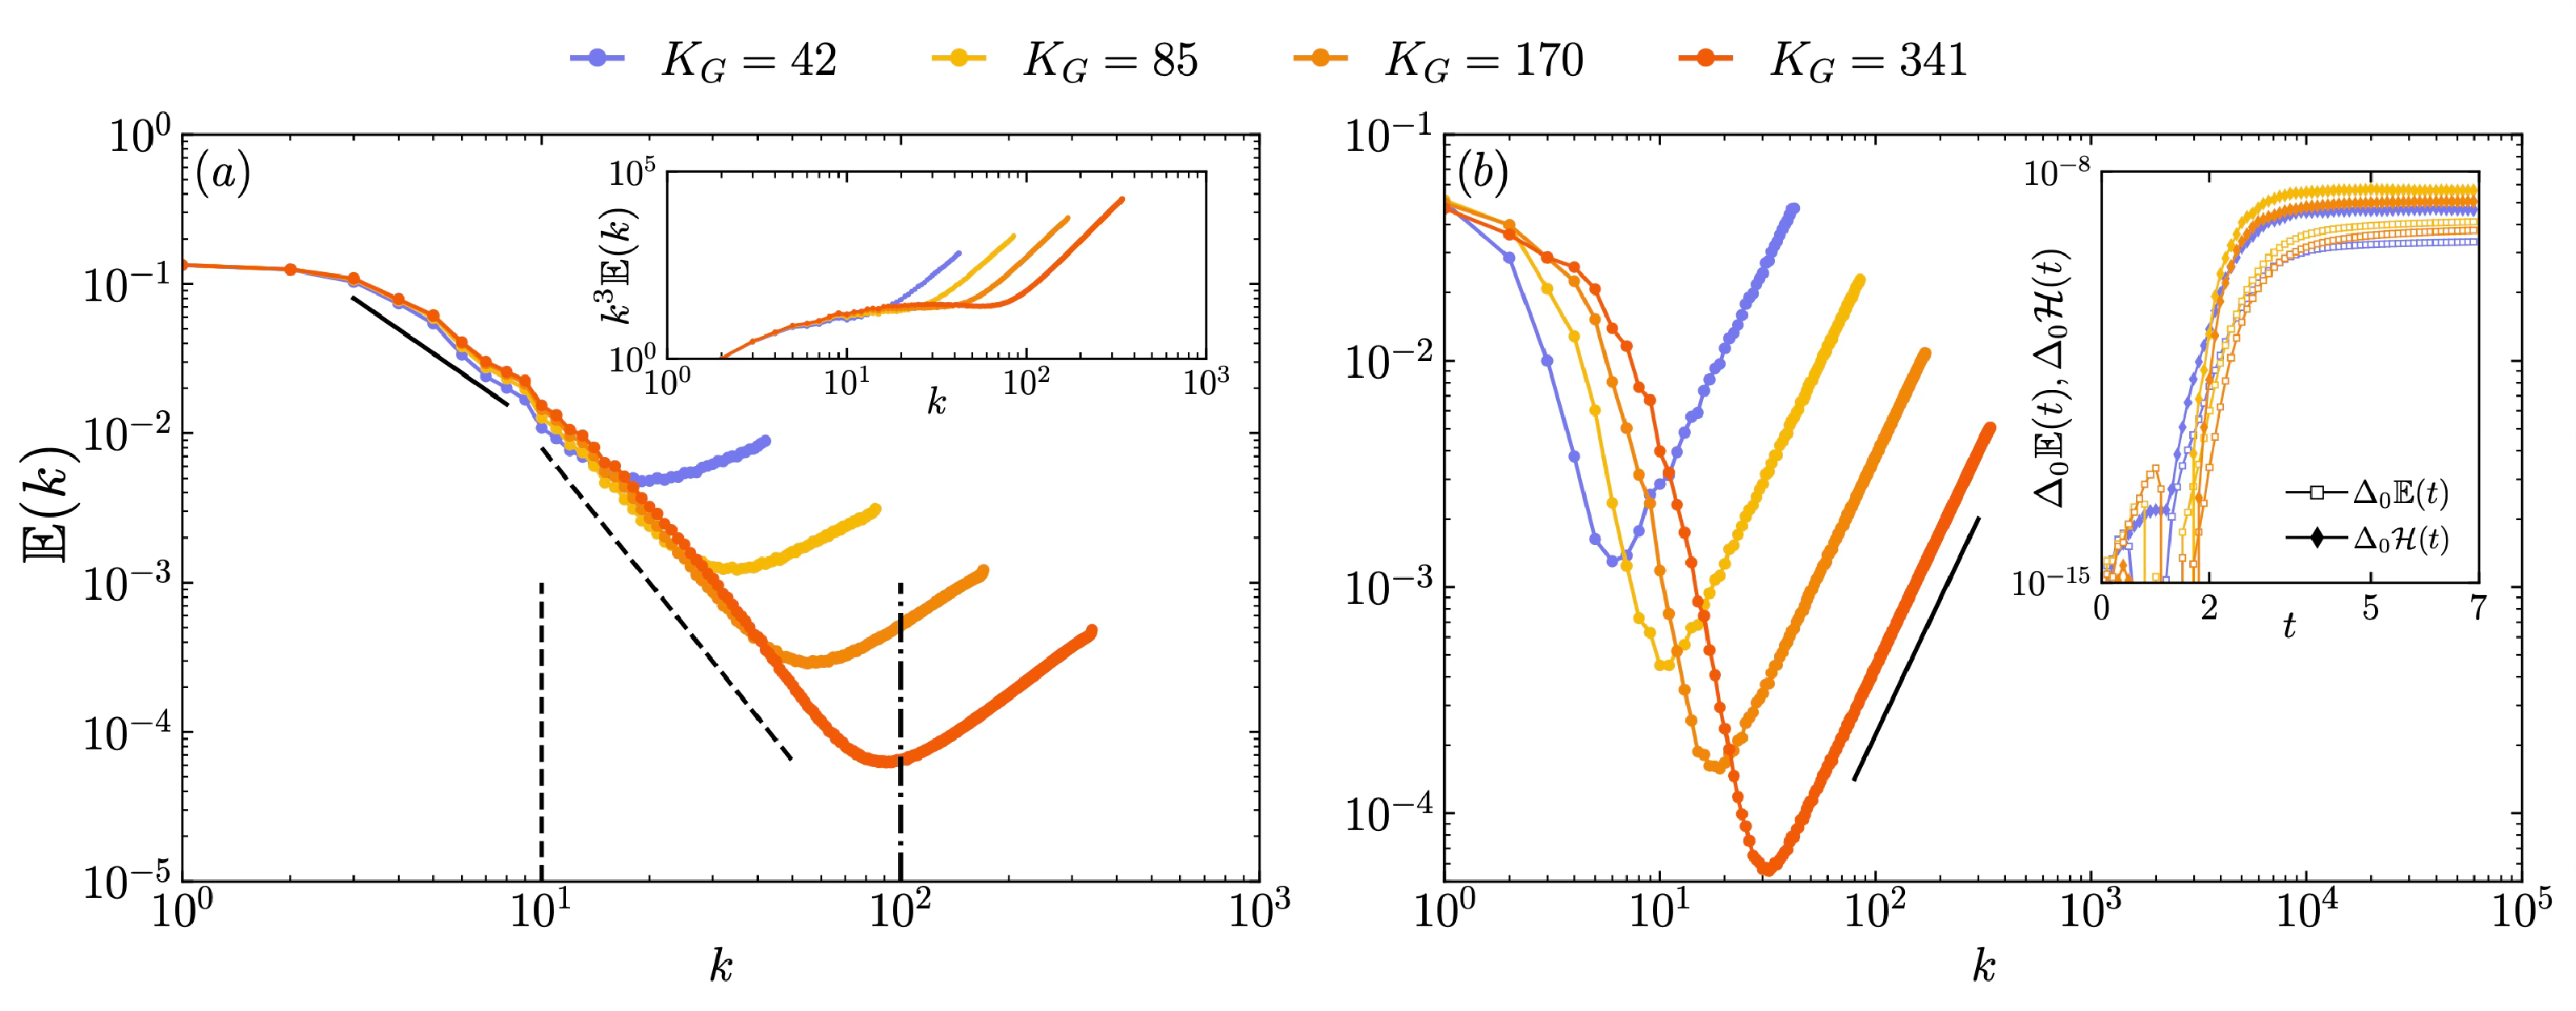
\includegraphics[width = \linewidth]{./figures/thermalization/Specra_allN_t3_t6.pdf}
	\caption[Energy spectra showing the $k^{-3}$ range and the partially thermalized state]{(a) Representative plot of the energy spectra, for different values of $K_{\rm G}$ (see legend) at $t = 3$.
	The (left) vertical dashed line corresponds to the wavenumber $K_{\rm I}$ marking the transition from a Kolmogorov-like
	$k^{-5/3}$ scaling  (indicated by the thick line as a guide to the eye) to one which follows a $k^{-3}$ scaling (indicated
	by a thick and a dashed line as guides to the eye). The $k^{-3}$ scale terminates and a pre-thermalised
	spectrum, with a positive slope, starts to develop. In the inset of panel (a), we confirm
	the pseudo-dissipation range $k^{-3}$ scaling
	through a compensated spectrum. At later times, such as $t = 6$ as shown in panel (b),
	the right tail follows a $k^2$ scaling as
	indicated by the thick line. {Inset of panel (b): time evolution of the
	relative errors in the energy and helicity,
$\Delta_0\mathbb{E}(t)=1-\mathbb{E}(t)/\mathbb{E}(0)$ and
$\Delta_0\mathcal{H}(t)=1-\mathcal{H}(t)/\mathcal{H}(0)$,
	showing that both remain conserved to high numerical accuracy.}}
	\label{thrm-fig1}
\end{figure}

As was shown by Cichowlas~\textit{et al.}~\cite{Cichowlasetal2005}, the large-scales of the flow, with $k \ll
K_{\rm G}$, follow a Kolmogorov scaling $k^{-5/3}$, indicated by the
dashed black lines in Fig.~\ref{thrm-fig1}(a). Indeed this Kolmogorov scaling persists even when
an equipartition spectrum kicks in as shown Fig.~\ref{thrm-fig1}(b). This suggests the co-existence
of a turbulent regime and a partially thermalised small-scales. However, the
$k^{-5/3}$ spectrum gives way to a pseudo-dissipation range with $\mathbb{E}(k) \sim
k^{-3}$ {(see Fig.~\ref{thrm-fig1}(a)). This is} consistent with findings
reported earlier that suggest a steeper-than-Kolmogorov intermediate wavenumber
scaling~\cite{Cichowlasetal2005,MuruganRay2023}. We observe that the $k^{-3}$ spectrum
is fairly robust (see the {inset of Fig.~\ref{thrm-fig1}(a)} with the
compensated spectrum $k^3\mathbb{E}(k)$) over a window of time --- the \textit{pre thermalised} phase ---
where (i) the first signatures of truncation by way
of a rising spectrum at large modes have appeared, and (ii) this rising spectrum is not yet equipartitioned.
We return to this question, and its possible explanation, in a subsequent section
of this manuscript.

This already suggests the existence of at least three time-scales. First, a cascade
completion time $t_{\rm cas}$ when the nonlinear transfers have led to the largest velocity modes $K_{\rm G}$
being non-zero unlike its initial $t = 0$ state. This is followed by a \textit{birth} timescale, $t_b > t_{\rm cas}$, when the first signatures of Galerkin-truncation, namely localised damped oscillatory structures~\cite{MuruganRay2023},
have appeared leading to an upturned, but not equipartitioned, energy spectrum at large modes.
A third timescale, $t_{\rm th} > t_b$, corresponds to when thermalisation sets-in with a clear $k^2$ spectral
range at the largest wavenumbers. Hence, in Fig~\ref{thrm-fig1}, panel (a) corresponds to times
$t_b \lesssim t \lesssim t_{\rm th}$ whereas panel (b) is at times $t \gtrsim t_{\rm th}$.
In a later section, we provide a heuristic way to estimate these timescales, and in particular their
dependence on the resolution $N_g$ of the simulation or, alternatively, the Galerkin wavenumber $K_{\rm G}$.
{The details of the direct numerical simulations which are used to address this question as well
as for Fig.~\ref{thrm-fig1} are described in Sec. 4.}

\section{Thermalisation: A brief review of the numerical studies}

Before we discuss the key results of our work, it is useful to briefly review
the numerical studies of the Galerkin-truncated Euler equation and the
understanding of thermalisation that have been developed so far.  The first
DNSs of such systems~\cite{Cichowlasetal2005}, similar to what we do here,
showed not just the phenomena of thermalisation but also that such partially
thermalised states, as shown in Fig.~\ref{thrm-fig1}, could serve as a
minimal model for turbulence with a $k^{-5/3}$ scaling range with the
thermalised small-scales acting as an effective thermal bath. Indeed, studies
soon after investigated in great detail the $K_{\rm th}$ transition wavenumber
as well as developed an effective two-fluid model to explain the coexistence of
absolute equilibrium thermalised (small-scale) states with a Kolmogorov-like,
self-similar (large-scale) turbulent
phase~\cite{BosBertoglio2006,KrstulovicBrachet2008,Krstulovicetal2009,Molfettaetal2015,MKV2023}.
More recently Murugan and Ray~\cite{MuruganRay2023} by using a combination of
specially curated flows --- such as vortex sheets and tubes --- along with more
generic initial conditions showed, in physical space, how thermalisation is
triggered locally in solutions of the Galerkin-truncated Euler equation, initially through small scale oscillation of wavelengths proportional to
$\nicefrac{1}{K_{\rm G}}$ which travel in directions normal to surfaces with
the largest velocity gradients. This work focussed on what we now identify as the pre thermalised phase.
In what follows, we identify the \textit{birth}
timescale $t_b$ associated with this pre thermalised solution. Eventually, these oscillations
interact to generate other harmonics and produce patchy regions of ``white-noise'' at times corresponding to $t_{\rm th}$ which account for the $k^2$
spectral tail.

The Galerkin-truncated 3D Euler equations are of course not the only ones which
thermalise. In fact, a more detailed understanding of how Galerkin-truncated
equations thermalise rests on a body of work which uses the one-dimensional
(1D) inviscid Burgers equation~\cite{Burgers1948} as the parent partial
differential equation. These studies were pioneered by Majda and
Timofeyev~\cite{MajdaTimofeyev2000} who showed the existence of a similar
equipartition spectrum for long time solutions of the truncated Burgers equation.
It was later discovered~\cite{RayetalTygers2011} how
shocks, integral to solutions of the inviscid partial differential equation,
lead to a resonance effect birthing spatially localised symmetric bulge-like
structures  --- christened \textit{tygers} --- at times $t_b \sim t_* - K_{\rm
G}^{-2/3}$ which eventually trigger thermalisation on timescales $t_{\rm th}
\sim K_{\rm G}^{-4/9}$~\cite{VenkataramanRay}.  ($t_*$ is the preshock time
where the inviscid Burgers equation admits it first real singularity.) Many
different aspects of these resonances, which are traced to finite-time blow-up
of the inviscid Burgers equation and the associated shocks, were studied
subsequently by several
authors~\cite{Pereiraetal2013,Leonietal2018,BrachetReview2022,Cartesetal2022,Kolluruetal2022,MKV2022}.

\section{Direct Numerical Simulations}

We perform direct numerical simulations (DNSs) of the Galerkin-truncated Euler
equation~\eqref{thrm-eq:GTE_FS} by using a fully-dealiased pseudo-spectral method
with a fourth order Runge-Kutta scheme for time-marching on triply-periodic
cube of length  $2\pi$. We consider five different resolutions with
collocation points $N_g^3 = 64^3, 128^3, 256^3, 512^3$ and $1024^3$. This allows us to
explore 5 different values of the Galerkin-truncation wavenumber, $21 \le
K_{\rm G} \le 341$. The time-step $10^{-3} \le \Delta t \le 10^{-4}$
is chosen separately for each resolution to ensure numerical stability. We choose an
initial (incompressible) velocity field ${\bf u}_0$ such that kinetic energy is concentrated at the
largest scales at $t = 0$. Our numerical scheme and choice of $\Delta t$ ensures that the
initial kinetic energy per unit mass $\mathbb{E}$ and Helicity $\mathcal{H}$ is conserved for all times, within numerical errors. {To verify this in our simulations, we compute the relative error
$\Delta_0\mathbb{E}(t)=1-\mathbb{E}(t)/\mathbb{E}(0)$ between the initial energy and its value at
time $t$. An analogous definition is used for the helicity
$\mathcal{H}$. The time evolution of these errors, shown in the inset of
Fig.~\ref{thrm-fig1}(b), demonstrates that both quantities remain
conserved to high numerical accuracy throughout the simulation.}

Somewhat paradoxically --- given the relative importance of the Euler equation ---  and unlike the 1D Burgers equation,
several questions remain open. Some of them, which  relate to the onset of thermalisation and indeed the
pre and partially thermalised phase illustrated in Figs.~\ref{thrm-fig1}(a) and (b), respectively,  are now addressed over
the next two sections.

\section{The $k^{-3}$ spectrum and {a constant Flux}}

We first investigate whether the self-similar form of the spectrum for
$k \lesssim K_{\rm th}$ is truly an \textit{``inertial''} range associated
with a constant energy flux $\Pi$. We also seek possible explanations of the origin of
the pseudo-dissipation range $k^{-3}$ scaling, for $K_{\rm I} \le k \le K_{\rm G}$, as seen in Fig.~\ref{thrm-fig1}(a).
It is important to caveat this by stressing that there is no {viscous}
dissipation in the Galerkin-truncated Euler equation. It is a conservative
system with a Hamiltonian description and conserves energy exactly. The thermalised scales do not dissipate but merely act as a thermal bath for the
larger scales to cascade its energy into. Our use of the word pseudo-dissipation
range is sociological and borrows from the terminology used in fully developed
turbulence for the transition scales between a $k^{-5/3}$ (up to intermittency
corrections) inertial range and the true exponential dissipation range.

Could the $k^{-3}$ scaling be universal for the pre-thermalised phase, and where
could it stem from? A possible, admittedly heuristic, explanation for this may
lie in the eddy-viscosity ideas of the two-fluid model proposed by Krstulovic
\textit{et al.}~\cite{Krstulovicetal2009}. Let $\mathbb{E}(k)$ be the yet undetermined
energy spectrum lying between the $k^{-5/3}$ (turbulence-like) and $k^2$
(thermalised) scales at wavenumbers $K_{\rm I} \le k \le K_{\rm G}$.
Dimensionally, and ignoring constants, the \textit{typical} velocities relate
to this spectrum as ${\hat u}^2_k \sim k\mathbb{E}(k)$. An  eddy-viscosity argument
leads to an eddy-damping timescale $1/\tau_d \sim \nu_{\rm eff} k^2$, where
$\nu_{\rm eff}$ is a phenomenological coefficient of eddy viscosity. This leads
to an effective dissipation $\epsilon \sim \nu_{\rm eff} k^2 {\hat u}_k^2$
which ought to be equal to a constant, so far hypothetical,  energy flux $\Pi$
that cascades from the large scale kinetic energy to the small-scale, thermalised
bath. Hence, $\Pi = \nu_{\rm eff} k^3 \mathbb{E}(k)$ from which the $k^{-3}$ scaling of
the pseudo-dissipation range follows.

{It is worth noting that, in our simulations, the spectra in this regime can
appear slightly steeper than $k^{-3}$. This steepening occurs very close to
the truncation scale $K_{\rm G}$, where the influence of the emerging thermalised
modes becomes significant. Given the limited spectral extent of this region
and the finite numerical resolution, it is difficult to make a definitive
statement about the precise scaling exponent. We therefore interpret this
behaviour as part of the crossover between the turbulence-like cascade and
the approach to the thermalised $\mathbb{E}(k)\sim k^{2}$ spectrum.}

Such an argument, while compelling, has several drawbacks. Most importantly, the idea
of an eddy viscosity for the pre-thermalised phase and not for the partially thermalised phase,
where we know the pseudo-dissipation range scaling is steeper than -3  (see Fig~\ref{thrm-fig1}(b)),
is somewhat puzzling in the absence of any strong argument to show relatively dominant Reynolds stresses
at timescales $t_b \lesssim t \lesssim t_{\rm th}$. Furthermore, the assumption of constant fluxes
seems marginally true. While for our largest simulations this constant flux is perhaps a persuasive
argument (see Fig.~\ref{thrm-fig2}(a)), the evidence for this is somewhat lacking for the lower resolutions
which nevertheless display the $k^{-3}$ scaling (see inset in Fig.~\ref{thrm-fig1}(a)). Hence we caution the
reader about the pitfalls of the argument we use to derive the numerically robust, pre-thermalised phase,
pseudo-dissipation range scaling, and a fuller theoretical understanding of this is warranted in future.

\begin{figure}
	% \includegraphics[width = 0.5\linewidth]{Fluxt3p0.png}
	% \includegraphics[width = 0.5\linewidth]{Fluxt6p0.png}
	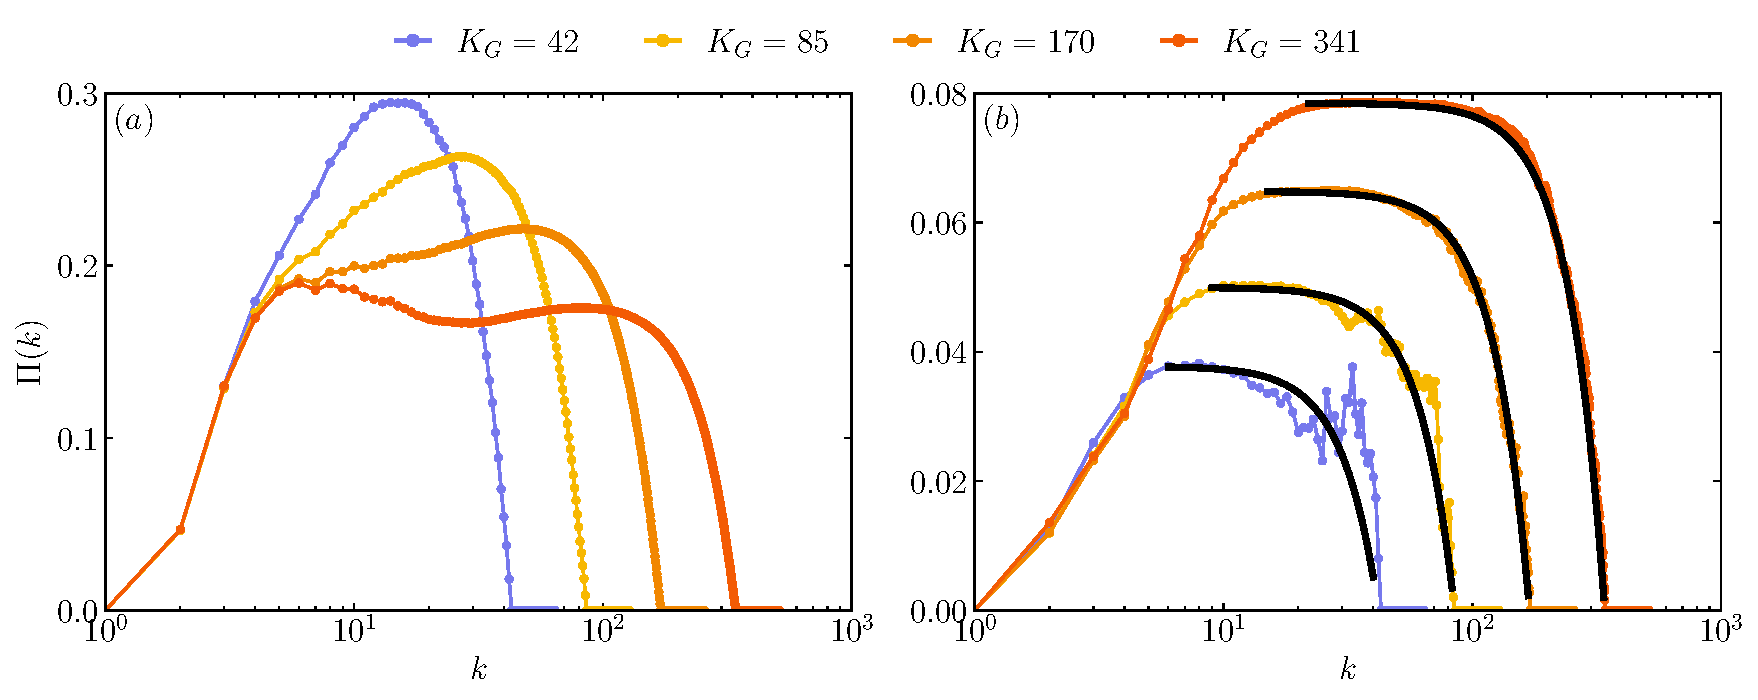
\includegraphics[width = \linewidth]{./figures/thermalization/Flux_allN_t3_t6.pdf}
	\caption[Energy flux for different Galerkin-truncation wavenumbers]{Representative plots of the energy flux, for different values of $K_{\rm G}$ (see legend), at (a) $t = 3$ and
	(b) $t = 6$. The solid black curve,  which overlay the data points in panel (b),
	are obtained from a theoretical estimate of $\Pi$ (see text) and provide a reasonable approximate of the flux for large $k$ and $K_{\rm G}$.}
	\label{thrm-fig2}
\end{figure}

One of the assumptions made above to understand the spectral scaling is that of a constant flux $\Pi$ across the
$k^{-5/3}$ and $k^{-3}$ scaling ranges. Is this really consistent with
measurements from our DNSs? In Fig.~\ref{thrm-fig2} we show $\Pi$ for all our
resolutions and at the same times for which we had shown the energy spectra in
Fig.~\ref{thrm-fig1}. At late times $t > t_{\rm th}$ we observe (Fig.~\ref{thrm-fig2}(b))
a remarkably robust, flat, $k$-independent plateau, indicating effectively an \textit{inertial} range
at scales larger than the thermalised scales. However at times $t_b \lesssim t \lesssim t_{\rm th}$,
as seen in (Fig.~\ref{thrm-fig2}(a)) and discussed in the previous paragraph, this constant flux regime
is less compelling.

Energy conservation allows us, nevertheless, to estimate the theoretical form
of the flux at least in the ultraviolet regime. Consider the partially
thermalised spectral form to be $\mathbb{E}(k) = \mathcal{C} k^2$, where $\mathcal{C}$ is a time-dependent
constant whose value can be estimated numerically. The nonlinear energy
transfer $T (k) = \frac{dC}{dt}k^2$ relates trivially to the time variation of
this spectrum, and which, in turn relates to the energy flux $\Pi (k) =
\sum_{k^\prime = k}^{K_{\rm G}}  T(k')\approx \nicefrac{1}{3}\frac{dC}{dt}\left [
	K_{\rm G}^3 - k^3\right ]$. In Fig.~\ref{thrm-fig2}(b), we overlay on
our DNSs data this theoretical curve
%(with $\frac{dC}{dt}$ obtained from the spectra measurements)
and find a convincing match with the flux
measurements from our simulations. However, at earlier times, such as the one shown in
Fig.~\ref{thrm-fig2}(a), this theoretical curve cannot predict the lack of a clear plateau at intermediate $k$.

\section{The Time-scales for Thermalisation}

We now address the question of the various timescales in the dynamics of
thermalisation and how they depend on $K_{\rm G}$. We recall that this question
was answered for the 1D Burgers equation, and the timescale $t_b$ and $t_{\rm
th}$ were estimated semi-analytically through the idea of
resonances~\cite{RayetalTygers2011} for the former, and Reynolds
stresses~\cite{VenkataramanRay} for the latter. Unfortunately, such tools are
not available at our disposal for the question of thermalisation in the Euler
equation~\cite{MuruganRay2023}. Furthermore, in this problem we also deal with
the cascade-completion time $t_{\rm cas}$, the analog of which for the Navier-Stokes
equation is a well studied
problem~\cite{Brachetetal1983,HerringKerr1993,RayetalEPJB}.

Let us begin with the cascade completion time $t_{\rm cas}$.  Given the initial
localisation of the kinetic energy in the first few wavenumbers $1 \leq k
\lesssim k_0$, where $k_0 \ll K_{\rm G}$, the nonlinear advection leads to
transfer of energy (and momentum) to wavenumbers $k > k_0$. We should thus be
able to construct a \textit{cascade} time scale $t_{\rm cas}$ which is a measure of the
time taken for the largest wavenumbers around $K_{\rm G}$ to be excited and
have finite, non-zero energies.

One way to estimate $t_{\rm cas}$ is through the time evolution of the enstrophy
$\mathcal{Z} = \sum_k k^2 \mathbb{E}(k)$. Given the sensitivity of the enstrophy to small-scale
excitations, $\mathcal{Z}$ grows in time as the energy cascade kicks in and higher
wavenumbers get excited. This process is consistent with what is known for
(decaying) simulations of the Navier-Stokes equation as well~\cite{Brachetetal1983}. However, there is
a critical difference. In the Navier-Stokes, $\mathcal{Z}$ reaches a maximum at
$t_{\rm cas}$ and subsequently decays with time as the total energy of the system
decays in the absence of
forcing~\cite{Brachetetal1983,HerringKerr1993,RayetalEPJB}. For our problem
this should not happen because of energy conservation and we ought to expect a
growth and saturation of $\mathcal{Z} \to \mathcal{Z}_\infty$ at late times.

In Fig.~\ref{thrm-fig3}(a) we show the time evolution of $\mathcal{Z}$ for
different resolutions.  Several things stand out. At short times the
curves collapse on top of each other till they start separating from the lowest
resolution onward. At long times the curves saturate to values
$\mathcal{Z}_{\infty}$ which depend on $K_{\rm G}$.

It is possible to theoretically estimate $\mathcal{Z}_{\infty}$. When the
flow is fully thermalised, the energy spectrum follows $\mathbb{E}(k) = \mathcal{C}_\infty k^2$, which, given the
conserved initial kinetic energy $\mathbb{E}_0$, allows for the determination
$\mathcal{C}_\infty = 6\mathbb{E}_0 [(K_{\rm G})(K_{\rm G}+1)(2K_{\rm G} + 1)]^{-1} \approx 3\mathbb{E}_0/K_{\rm G}^3$, for large $K_{\rm G}$.
By using this, it is trivial to show that, for large $K_{\rm G}$,  the
saturation value $\mathcal{Z}_{\infty} =  \nicefrac{3}{5}\mathbb{E}_0 K_{\rm G}^2$. In Fig.~\ref{thrm-fig3}(a) we plot
$\mathcal{Z}_{\infty}$, as dashed horizontal lines, to see how the system evolves to
the fully thermalisation phase.

Unlike the Navier-Stokes equation, $\mathcal{Z}$ is not an ideal
metric for estimating $t_{\rm cas}$. Of course, one possibility is to estimate the time when
the curves for different values of $N_g$ separate from the collapsed curves at short times as
seen in Fig.~\ref{thrm-fig3}(a). Consistent with intuition, a time-scale obtained from this observation
grows with $N_g$. However, there is a drawback to using this prescription: It does not allow us to determine
$t_{\rm cas}$ for the largest resolution since this measurement is, by definition, relative to the $\mathcal{Z}$ curve
for $N_g = 1024$.

A more natural way to think about $t_{\rm cas}$ is to estimate the time when the kinetic
energy for the largest mode is non-zero. This would correspond to a
culmination of the cascade process whence all scales have been excited.
Numerically, for $t < t_{\rm cas}$, the energy of the largest mode in the kinetic
energy spectrum $\mathbb{E}(K_{\rm G})$ is below the machine precision value. We now
record the time $t_{\rm cas}$ when this threshold is crossed. Of course the estimation of $t_{\rm cas}$
is somewhat inaccurate in simulations where the data is saved at discrete time intervals. Nevertheless, within such an approximate approach, we evaluate the
cascade-completion time-scale $t_{\rm cas}$, and find, in Fig.~\ref{thrm-fig3}(b), a
logarithmic scaling of $t_{\rm cas} \sim \log N_g$.

The cascade completion time $t_{\rm cas}$ does not indicate the onset time for thermalisation, $t_{\rm th}$, or indeed the time $t_b$ at which the precursor to thermalisations show up:
$t_{\rm cas} < t_b < t_{\rm th}$.  Murugan and Ray~\cite{MuruganRay2023} had shown that
for the truncated Euler equations the first signs of the solution being
\textit{different} from $\nu \to 0$ Navier-Stokes solutions are localised,
monochromatic oscillatory structures which emerge \textit{out of the blue} in
physical locations proximate to structures with the steepest gradients. These
structures, constituting the pre-thermalised phase, are \textit{born} at times $t_b$ and eventually trigger
thermalisation with the energy for modes beyond $K_{\rm th}$
equipartioned at times $t \gtrsim t_{\rm th}$. This two-step trigger, resulting in a dual timescale,
is reminiscent of thermalisation
in the one-dimensional Galerkin-truncated Burgers equation.

We test this idea on the data from our DNSs. Careful observations suggest that
at times soon after $t_{\rm cas}$, well before the first signs of an incipient
equipartition spectrum is detectable, the $k^{-3}$ scaling extends all the way
to $K_{\rm G}$. In time, the ultra-violet end of the spectrum starts to bend
upward, but not yet equipartitioned, over a time window $t_b \leq t \lesssim
t_{\rm th}$ constituting the pre thermalised phase.  We see an example of this
in the inset of Fig.~\ref{thrm-fig3}(b).

\begin{figure}
	% \includegraphics[width = 0.32\linewidth]{enstrophyvstime.png}
	% \includegraphics[width = 0.32\linewidth]{time_scalestbtc.png}
	% \includegraphics[width = 0.32\linewidth]{gamma.png}
	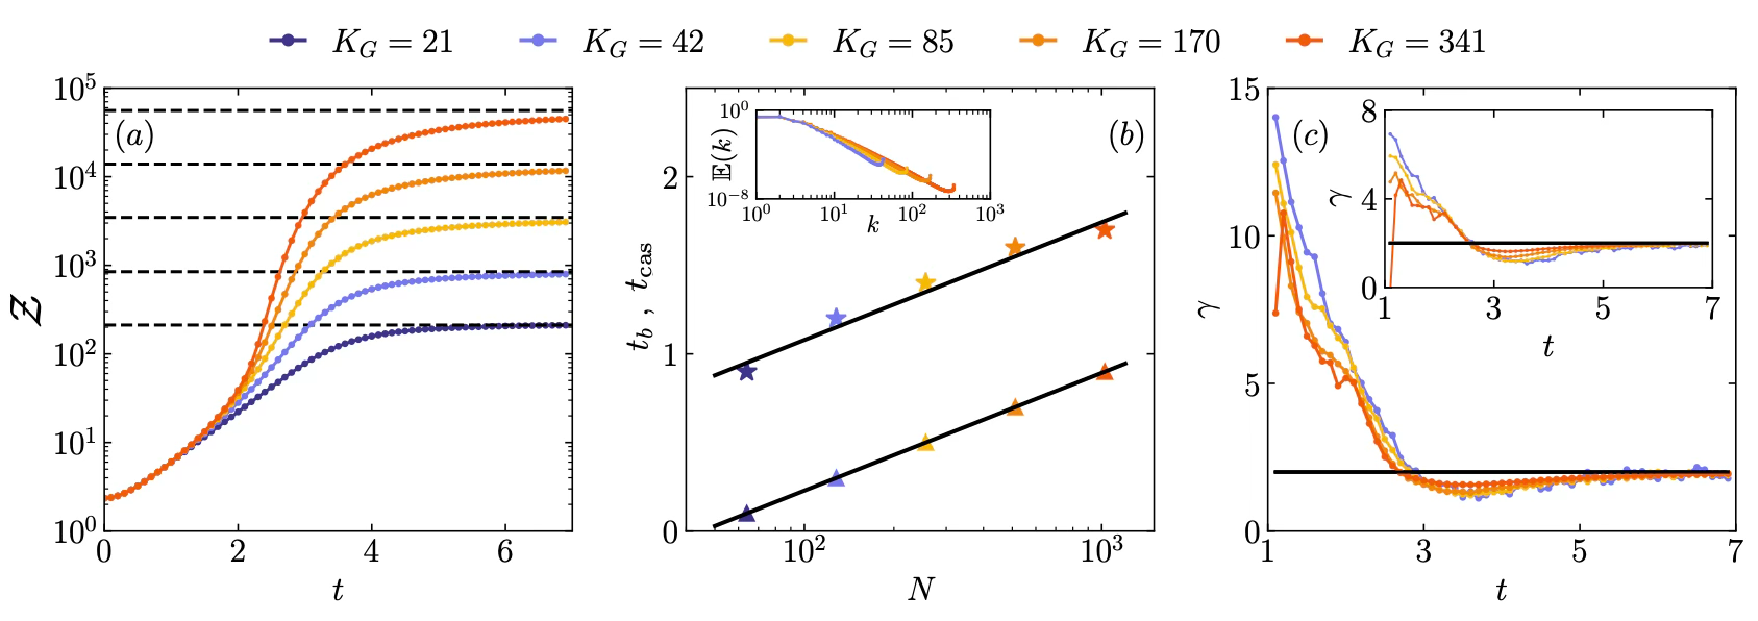
\includegraphics[width = \linewidth]{./figures/thermalization/enstrophyvstime_time_scalestbtc_gamma.pdf}
	\caption[Enstrophy growth, cascade timescales, and the thermalization timescale]{(a) A plot of the enstrophy $\mathcal{Z}$ versus time for different Galerkin-truncation wavenumbers $K_{\rm G}$ showing the growth
	and $K_{\rm G}$ dependent saturation at $\mathcal{Z}_\infty$, indicated by the horizontal dashed lines (see text). At short times the curves
	for different $K_{\rm G}$ collapse, and as smaller scales get excited, they separate.
	(b) The timescales for cascade completion $t_{\rm cas}$ (triangles), and the \textit{birth} $t_b$ (stars) of the localised oscillatory structures which eventually trigger thermalisation plotted against $N_g$. The linear curves in the semilog plot suggest that both these timescales depend
	logarithmically on $N_g$. The inset shows the energy spectrum, for different $N_g$, or equivalently for different $K_{\rm G}$, at $t_b$ showing the departure at the ultraviolet end from
	the $k^{-3}$ scaling before the onset of an equipartition $k^2$ spectrum. (c) The variation of the spectral slope $\gamma$ (see text) for wavenumbers {within a range $\mathcal{X}K_{\rm G} < k < K_{\rm G}$ with $\mathcal{X} = 10\%$}. The horizontal dashed line indicates a slope of 2 corresponding to the
	equipartition $\mathbb{E}(k) \sim k^2$ spectrum. In the inset we
	show the analogous result for $\mathcal{X} = 15\%$ leading to the same conclusion.}
	\label{thrm-fig3}
\end{figure}

A simplistic formulation of when the $k^{-3}$ gives way to a rising
spectrum in the pre thermalised phase is to estimate
the time $t_b$ at which the energy of the largest mode $\mathbb{E}(K_{\rm G}) \gtrsim C
K_{\rm G}^{-3}$. The time-dependent constant $\mathcal{C}$ is
obtained from our data.  We find from such measurements that $t_b \sim
\log N_g$, illustrated in Fig.~\ref{thrm-fig3}(b), just like the scaling form for $t_{\rm cas}$, but with a
different prefactor since $t_b > t_{\rm cas}$.

We finally consider the thermalisation timescale $t_{\rm th}$. Unlike the
resonance conditions and consequent Reynolds stress triggered collapse from a
monochromatic to white noise form for the 1D Burgers equation, theoretical
progress is difficult in {the Galerkin-truncated Euler} problem. We therefore resort to the following
ad-hoc measure.

{We consider a range of the largest wavenumbers, lying between $\mathcal{X} K_{\rm G} \le k \le K_{\rm G}$,
such that its extent is a percentage $\mathcal{X}$ of the Galerkin-truncation
wavenumber $K_{\rm G}$. If we measure the spectral slope of $\mathbb{E}(k) \sim k^\gamma$ for this range of wavenumbers, $\gamma \to 2$ as
$t \to t_{\rm th}$. Of course, it is neither obvious nor necessary (for this calculation) that the spectrum in this range is
necessarily a power-law; what matters is that as these wavenumbers thermalise, their energy ought to scale as $\mathbb{E}(k) \sim k^2$.}

In Fig.~\ref{thrm-fig3}(c), we show a plot of $\gamma$ vs time, with
$\mathcal{X} = 10\%$, for different values of $K_{\rm G}$. The $\gamma \neq 2$
range is irrelevant for the reason discussed above. What is important is how
$\gamma$ approaches 2 for different $K_{\rm G}$. Within statistical errors in the
measurement of $\gamma$, our results suggest that $t_{\rm th}$ is independent
of or only weakly dependent on $K_{\rm G}$. %This suggests that the thermalisation time $t_{\rm th}$ is, unlike the 1D Burgers problem, independent of $K_{\rm G}$.
{This is unlike what is known for the analogous  problem in the 1D Burgers equation where the thermalization timescale scales as $K_{\rm G}^{-4/9}$~\cite{VenkataramanRay}}.

It useful to add a caveat here. While ideally, the time for the onset of
thermalisation ought to be estimated with as small a percentage $\mathcal{X}$
as possible, a numerically trustable fit over a self-similar spectrum
constrains us on the smallest  $\mathcal{X}$ that we can practically use.
Thus we confirm the conclusion $t_{\rm th} \sim K_{\rm G}^0$ by varying
$5\% \le \mathcal{X} \le 20\%$; in the inset of Fig.~\ref{thrm-fig3}(c) we
show a plot of $\gamma$ for $\mathcal{X} =  15\%$ which leads to same conclusion as before.

\section{Outlook \& Perspective}

As we conclude, let us address the question of the relevance of such studies
for turbulence and statistical physics. While a detailed review of this
is beyond the scope of the present paper, let us offer some perspective
on this question.

The nature of thermalised solutions would lead one to believe that these
systems have very little to do with turbulence. This is only partially true.
For problems more directly relevant to natural or experimental turbulent flows,
one of the successes of such solutions has been in providing
\textit{an} explanation~\cite{FrischetalBottleneck2008,FrischetalBottleneck2013}
for the bottleneck phenomenon~\cite{Falkovich1994,Lohse1995}. A bump between the
inertial and dissipative ranges in the compensated $k^{5/3} \mathbb{E}(k)$ energy
spectrum in turbulence~\cite{Pak1991,SheJackson1993,Gotohetal2002,Kurien2004,Verma2007,Mininni2008,Ishihara2009,Donzis2010}.

Numerical simulations have confirmed how such effects are exaggerated with the use of hyperviscosity \cite{FrischetalBottleneck2008,BanerjeeRayHyperviscosity2014}
instead of the regular Laplacian
dissipative term.  Such explanations lie in the observation that
higher-order hyperviscous terms will converge to the Galerkin-truncated
equation~\cite{FrischetalBottleneck2008,BanerjeeRayHyperviscosity2014} and hence lead to the non-monotonic
energy pile up --- bottleneck --- between the inertial and far dissipation ranges.
Likewise, a more generalised form of the Galerkin projection --- the so-called
decimation projector~\cite{FrischetalDecimation2012} --- have been used to
address questions of
intermittency~\cite{Lanotte2015,Buzzicottietal2016Burgers,Buzzicotti2016NS} and
irreversibility~\cite{Ray2018,Picardoetal2020} which remain central to the
statistical physics and statistical field theory of turbulence. These ideas have been further
supplemented by studies related to entropy in the partial and fully thermalised
regimes of such equations~\cite{MKV2024}.

A more involved aspect of studies of Galerkin-truncated systems comes from numerical
investigations for potential finite-time singularities in the Euler equation
which inevitably tackle such questions. This is because a spectral (numerical) approach to solving equations such as the Navier-Stokes for turbulence naturally lead to solving the Galerkin-truncated equation when $\nu = 0$.
Hence, as reported by Bustamante and Brachet~\cite{BustamanteBrachet2012}, and
more recently for the axisymmetric problem by Pandit and collaborators~\cite{Kolluruetal2022,KolluruPandit2024,KolluruetalJCP2024},
singularity tracking through techniques such as the analyticity strip
method~\cite{Sulemetal1983} would invariably encounter the effects of
thermalisation. {Indeed, this provides a key motivation and so
far an open problem of how to circumvent or indeed delay the onset of
thermalisation and recover possible dissipative solutions of the Euler
equation. So far, such attempts have been restricted to very special cases for
the Euler equation~\cite{MuruganRay2023,Fehnetal2022,Fargeetal2017}; these
include, for example, the suppression of resonant structures responsible for
triggering thermalisation in truncated Euler flows~\cite{MuruganRay2023},
wavelet-based regularisation and denoising procedures which selectively remove
such small-scale oscillations~\cite{Nguyen2009,Fargeetal2017,Pereira2022,PereiraSIAM2023}, and numerical studies
suggesting the emergence of dissipative behaviour in carefully designed
inviscid simulations~\cite{Fehnetal2022}.} This is unlike the 1D Burgers
equation where a more concrete theory of how such questions can be tackled have
been reported~\cite{Muruganetal2020,Kolluruetal2024}. We hope that our work on
the dynamics of thermalisation may spur more efforts in such directions. One
possibility would be to identify in a coarse-grained manner, such as the one
developed recently for the Navier-Stokes multifractality
problem~\cite{Mukherjeeetal2024}, how inhomogeneous is the distribution of the
trigger points of thermalisation. This may well lead to a numerical
prescription on how these spots can be selectively eliminated.  Finally, for
the Galerkin-truncated Euler equation to serve as a sub-grid scale model for
turbulence, inertial range intermittency through measurements of the equal-time
scaling exponents, for example, in the $k^{-5/3}$ scaling range in the
partially thermalised phase, needs further investigation.

\enlargethispage{20pt}

\subsection*{Data accessibility}
The data from our numerical simulations are available on request.

% \subsection*{Competing interests}
% The authors declare that they have no competing interests.

% \subsection*{Funding}
% SSR acknowledges the Indo–French Centre for the Promotion of Advanced
% Scientific Research (IFCPAR/CEFIPRA, project no. 6704-1) for support. The simulations were performed on the ICTS Contra cluster.
% CR, MSK, and SSR acknowledge the support of the Department of Atomic Energy,
% Government of India, under project no. RTI4019.

\subsection*{Acknowledgements for this work}
The authors thank R. Mukherjee and S. Sahoo for several useful discussions. CR thanks A. Sherry, J. Kethepalli, and T. Ray for their insights. The code used to generate the data is hosted publicly on \href{https://github.com/Rajarshi-prime/GT-Euler}{GitHub}. Microsoft and GitHub copilot were used for code development and plot formatting.

\end{document}
